\documentclass[12pt,fleqn]{article}
\setlength{\parindent}{0pt}
\usepackage{graphicx}
\usepackage{listings}
\usepackage[latin5]{inputenc}
\setlength{\parskip}{8pt}
\setlength{\parsep}{0pt}
\setlength{\headsep}{0pt}
\setlength{\topskip}{0pt}
\setlength{\topmargin}{0pt}
\setlength{\topsep}{0pt}
\setlength{\partopsep}{0pt}
\setlength{\mathindent}{0cm}

\begin{document}
MIT OCW Cok Degiskenli Calculus - Ders 10

Bugunku konumuz kritik noktalarin minima mi, maksima mi, yoksa eger noktasi
mi oldugunu anlama teknikleri. Kritik noktalar kismi turevlerin hepsinin
sifir oldugu noktadir, mesela 2 degiskenli fonksiyon icin $f_x=0$, $f_y=0$
olmalidir. 

3 degisik kritik nokta cesidi gorduk, lokal minima, lokal maksima, ve
eger (saddle) noktalari. 

Bir fonksiyonun birden fazla kritik noktasi olabilir. Mesela soyle bir
fonksiyon

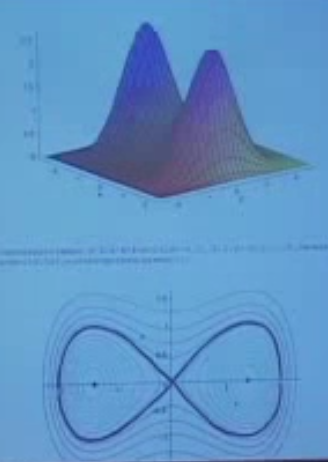
\includegraphics[height=4cm]{10_1.png}

Soru: Bir kritik noktaya bakarken, hangi kategoriye ait oldugunu nasil
anlayacagiz? Bir diger soru, global (lokal olmayan) minimum ve maksimum
noktalarini nasil buluruz?  Ustteki resimdeki fonksiyonda iki lokal
maksimum var. Her ikisini de deneyebiliriz, hangisi daha yuksek ise onu
aliriz. Diger yandan, bu fonksiyonun minimumu herhangi bir ``noktada'' degil,
maksimumdan uzakta, fonksiyonun en dis yerlerinde, sonsuzlukta. 

Yani global minimum ve maksimum illa bir noktada olmayabilir, sonsuzlukta
olabilir, o zaman bu kosulu test etmeliyiz, fonksiyonumuzun sonsuzluga
giderken nasil davrandigini anlamaliyiz.

Birinci soruyu cevaplayalim

Ikinci Turev Testi

$w = ax^2 + bxy + cy^2$

Bu fonksiyonun kritik noktasi orijinde. Eger turevleri alirsak, ve sifira
esitlersek, sonuc $x,y=0$ cikar. Ayni sekilde eger $w$'nin lineer
yaklasiksallamasini yapsaydik esitlik sagindaki butun terimlerin $x,y$
kucuk iken $x,y$'den kucuk oldugunu goruruz, o zaman grafigin tegeti $w=0$
noktasindadir. Eger orijinden ufak bir adim atarsak, o adimlarin fonksiyon
uzerindeki etkisi kare alma operasyonu yuzunden daha kuculur ($0.001^2 =
0.00001$ 
mesela). Herhangi bir noktadaki egim fonksiyon / degiskenlerdeki artis
olduguna gore, orijine yakin olan egim yukari dogru neredeyse yok gibidir. 

Ornek

\[ w = x^2 + 2xy + 3y^2 \]

Ustteki formulu su sekilde donusturursek

\[ w = (x+y)^2 + 2y^2 \]

Ustte iki karenin toplami var, karelerin ikisi de negatif olamaz, o zaman
minimum'un orijin olmasi gerekir (negatiflesmeden olabilecek en kucuk deger
oradadir). 

Birazdan gorecegiz ki ustteki kare tamamlama (completing the square)
yontemini $a,b,c$ katsayilarini iceren genel durum icin de kullanabiliriz. 

Once $a \ne 0$ farz etmem lazim, yoksa teknigin geri kalani mumkun olmaz. 

\[ w = a \bigg( x^2 + \frac{b}{a} xy \bigg) + cy^2 \]

Eger bir kare denklemin orta teriminde $b/a \ xy$ (ustteki gibi) elde etmek
istiyorsam, kare icinde $x$ ve $b/2a \ y$ terimlerini kullanirim, cunku bu iki
terimin birbirleri ile carpilip iki kere toplanmalari $b/a \ xy$ sonucunu
verir. O zaman

\[ = a \bigg( x + \frac{b}{2a}y  \bigg)^2  + ... \]

Hala isimiz bitmedi, kare icine koyulan $y$ yuzunden ortaya cikan $y^2$ bazli
terimi dengelemek gerekiyor,

\[ = a \bigg( x + \frac{b}{2a}y  \bigg)^2  + 
\bigg( c - \frac{b^2}{4a} \bigg)y^2
 \]















\end{document}
